%ब
\chapter{Design of Referential Integrity Constraints in NoSQL
databases} \label{c:solutions}

% As mentioned previously,    cloud column-oriented key-value \acp{DBMS} lack
% referential integrity constraints to maintain foreign key relationships,    as
% seen in traditional \acp{RDBMS},    due to its non-relational data model.    
% Moreover,    these cloud \acp{DBMS} do not normalise data nor maintain
% relationships.   
Traditionally,   referential
integrity constraints are imposed on data items of a database to maintain
foreign key relationships.    These relationships are
 maintained by correctly identifying and preserving the data dependencies 
 existing between the data items.   
% Traditionally,   foreign key relationships are
% maintained by correctly identifying and preserving the data dependencies existing between data items in a database.   
% These dependencies are maintained and  validated by imposing referential
% integrity constraints on data items.    
Most popular traditional \acp{RDBMS}
preserve such dependency information in their \texttt{System} tables or data
dictionaries.     These tables store the necessary information  which is required
to maintain valid dependencies.    The information stored in such tables include table
names,    primary and foreign keys,  among others.   
This can be seen in popular \acp{RDBMS} like  MS SQL Server,    PostgreSQL,  
Oracle,   and so on.     

For example,    in MS SQL Server 2000,   \texttt{sysforeignkeys} is a
\texttt{System} table which stores the information of all foreign keys of every
table in a database,   and \texttt{sysreferences} stores the mappings of  foreign
keys to the referenced primary key columns \citep{msdn}.  Information in these
\texttt{System} tables consist of  the names of tables and its constraints, 
unique identifiers of referenced and referencing columns and others.  In
PostgreSQL,   such information is presented to users as views but it is stored in
base tables which contain the dependency information of data items in a
database.  The view \texttt{table\_constraints} show the information about all
the constraints in every table owned by the current user~\citep{postgres}. 
Similarly,   Oracle uses a \texttt{SYSTEM} meta-database to hold such constraint
information.   In general,   \texttt{System} tables or views with information
about the existing dependencies  are looked up by these \acp{RDBMS} whenever
referential integrity checks are triggered \citep{msdn}. 


The solutions presented in this thesis save the dependency information as
metadata.    This metadata contains relevant  information about primary keys of
column families and foreign key relationships in keyspaces.   Thus,  metadata is
accessed whenever an operation is performed on the data and referential
integrity needs to be validated.  These solutions are implemented using an
experimental \ac{API} which is discussed in Chapter~\ref{c:Implementation}. 


This chapter presents the design of  four  solutions  that implement referential
integrity constraints in a cloud \ac{NoSQL} \ac{DBMS}.   
Section~\ref{s:design-Metadata} describes the metadata used by the solutions 
 to store the dependency information.    Sections~\ref{s:design-sol1}, 
 ~\ref{s:design-sol2}, ~\ref{s:design-sol3}, ~\ref{s:design-sol4}  present
 the design and motivation of the four solutions. 
%  of the first solution.   
%  Section presents Solution~2 and its design and motivation.    Section describes the design
%  and motivation of Solution 3.    Section presents the design
%  and motivation of Solution~4.   
Section~\ref{s:Design-summary}
 summarises the design of the four solutions.   
 % Section~\ref{s:API} describes the design and implementation of the experimental
% API developed to integrate all the four
% solutions.    
% Section~\ref{s:sol1} describes  the first solution,   which implements
% referential integrity constraints by saving metadata along with the actual data.   
% Section~\ref{s:sol2} describes the second  solution where metadata is
% saved as a top row.    Section~\ref{s:sol3} describes the third   
% solution which saves metadata separate from the actual data.      
% Section~\ref{s:sol4}  describes the fourth solution which saves metadata in a separate cluster.   
% Finally,   Section~\ref{s:solutions-summary} presents a brief summary of this
% chapter.    

% ब
\section{Metadata}\label{s:design-Metadata}
Metadata in \acp{DBMS} provide information about the data stored within the
databases.
It may contain details related to schemas, constraints,  primary and foreign
keys, and so on.   As previously mentioned,  most traditional \acp{RDBMS}
maintain such metadata within their \texttt{System}  tables or data
dictionaries.
In Apache Cassandra, the \ac{DBMS} of interest, metadata is stored in a keyspace
named \texttt{System} and it contains information about the cluster and its
nodes along with information related to the keyspaces, column families, and so
on~\citep{BOOK}.
 Even when Cassandra has a  \texttt{System} keyspace to store metadata, it is
 read-only and therefore it cannot be modified to store additional metadata
 about referential integrity constraints.
% As previously mentioned ,  most traditional \acp{RDBMS} maintain such metadata
% within their \texttt{System} tables or data dictionaries.
% Such metadata is decoupled from the actual data and its operations,  so that
% retrieving the metadata is faster since it does not involve handling the
% actual data(\todo{cite Duval}).
% It has been studied that the \ac{DaaS} is moving towards maintaining metadata
% in the cloud \acp{DBMS},  where commonly this metadata stores information
% about the nodes in a distributed cluster (\todo{cite Bin(2010)}).  For 
% maintaining the scalability required in such cloud \acp{DBMS}, metadata is
% often decoupled from the actual data so that accessing metadata does not cause
% a bottleneck in performance.  Cassandra maintains  metadata about the nodes in
% a cluster  in a separate keyspace named \texttt{System}, which stores the
% properties of every node, for example the node tokens,  the name of the
% cluster to which  nodes belongs to, information about the stored keyspaces and
% column families and so on(\todo{cite BOOK}).
% As per the design of Cassandra,  the \texttt{System} keyspace cannot be
% modified and thus  the metadata for the   solutions cannot be incorporated in
% this \texttt{System} keyspace.  Hence,  for preserving the metadata in each
% solution implements a  different strategy In other words, metadata is
% associated with actual data in different ways.  Associations can be classified
% as (\todo{cite Duval}):
Hence,  for preserving the metadata, each of the solutions implement a 
different strategy in which metadata is associated with actual data. Solutions~1
and~2 use embedded metadata, that is, metadata is created with the actual
data; while solutions~3 and~4 associate metadata separately from
the actual data.  Notice that, the structure of the metadata is kept the same across all the solutions even when  the way of
 storing and associating this metadata is different in each.

The role of metadata in  the solutions is primarily to hold the necessary
 information required to maintain referential integrity. The metadata contains
 information about primary keys,   foreign keys,  referenced and referencing
 column family details, constraints, and others.  The constraints considered in
 the solutions can be either \ac{PK} or \ac{FK} constraints. \ac{PK} constraints
 specify which column is the primary key of a column family. \ac{FK} constraints
 (or referential integrity constraints) determine the foreign key relationship
 between two column families, that is, the column of a column family which  is
 dependent on the primary key  column of another column family.  Hence, for each
 column family with a primary key,  the metadata  contains one \ac{PK}
 constraint  and  as many \ac{FK} constraints as foreign key relationships the
 column family has.
% Notice that, throughout the solutions, the structure of metadata containing
% these constraints is consistent despite.

The structure of the metadata is shown in Figure~\ref{fd:Metadata-Constraints}.
This structure contains information about a University keyspace example in which
 a simple schema is applied for the keyspace. In this example,  the details of
the students are saved in  the \texttt{Student} column family and the course
 details in the \texttt{Course} column family.  The enrolment details of
 students are saved in the \texttt{Enrolment} column family by associating
 students to courses and hence having foreign key relationships to both
 \texttt{Student} and \texttt{Course} column families. All the column families
 have unique primary keys and their \ac{PK} constraints are saved in the
 metadata as presented in Figure~\ref{fd:Metadata-Constraints} while the foreign
 key relationships between \texttt{Enrolment}, \texttt{Student} and \texttt{Course} are saved as \ac{FK} constraints.  For instance, consider in
 Figure~\ref{fd:Metadata-Constraints} the \ac{PK} constraint \texttt{CONST100},
 for the \texttt{Student} column family, and the \ac{FK} constraint
 \texttt{CONST400} for the foreign key relationship between
\texttt{Enrolment} and \texttt{Student}. Notice that only
 single column primary keys are considered in the solutions.

\begin{figure}[h] 
	\centering
	
	\newcolumntype{C}{@{\hspace{2.5pt}}>{\scriptsize}c@{\hspace{2.5pt}}}
	\begin{tabular}{CCC CCC CC}
		\toprule
		\bfseries ConstraintName & \bfseries Keyspace & \bfseries ConstraintType &
		\bfseries ColumnFamily & \bfseries RKeyspace & \bfseries RConstraintName &
		\bfseries RColumn & \bfseries DeleteRule\\
		\midrule
		CONST100 & University & P & Student & University & & StudentId &\\
		\rc CONST200 & University & P & Course & University & & CourseId &\\
		CONST300 & University & P & Enrolment & University & & RowId &\\
% 		\hline
% 		\hline
		\rc CONST400 & University & R & Enrolment & University & CONST100 & StudentId
		& CASCADE\\
		CONST500 & University & R & Enrolment & University & CONST200 & CourseId &
		NODELETE\\
		\rc CONST600 & University & F & Course & University & CONST500 & CourseId &
		NODELETE\\
		CONST700 & University & F & Student & University & CONST400 & StudentId &
		CASCADE\\
		\bottomrule
	\end{tabular}
	\caption{Metadata for the Solutions}\label{fd:Metadata-Constraints}
\end{figure}


Specifically, the structure of the metadata contains:

\begin{itemize}
  
  \item \texttt{ConstraintName:} is the name assigned for
  every constraint and it uniquely identifies an
  existing \ac{PK} or \ac{FK} constraint in the metadata. 
   For example,  \texttt{CONST100} and \texttt{CONST400} are 
  \texttt{ConstraintNames}.
  
  \item \texttt{Keyspace:}represents the name of the Keyspace the constraint
  belongs to. 
  
  \item \texttt{ConstraintType:} denotes the type of the constraint and the
  possible values are '\texttt{P}', '\texttt{R}' and '\texttt{F}'.
% The former referes to  a \ac{PK} constraint while the latter represents  a
% \ac{FK} constraint.
	A \ac{PK} constraint is referred by '\texttt{P}', while '\texttt{R}' and
	'\texttt{F}' are two representations of \ac{FK} constraints.
	'\texttt{R}' represents the referential integrity constraint (or  \ac{FK}
	constraint) a child entity has on a parent primary key, and '\texttt{F}'
	represents the  existing dependencies on a parent entity . For example,
	\texttt{CONST400} shows that the  parent entity for \texttt{Enrolment} is
	\texttt{Student} by looking up \texttt{RConstraintName}.
	\texttt{CONST700} shows that parent entity \texttt{Student} has child
	dependencies on it by following \texttt{CONST400}. Notice that, the constraint
	type '\texttt{F}' is primarily used to locate the child dependencies for a
	parent when it is deleted or updated.
% \begin{itemize} \item  '\texttt{P}' represents a \ac{PK} constraint \item
% '\texttt{R}' represents a

   
  \item \texttt{ColumnFamily:} refers to the column family this constraint
  applies to. For example,  the \ac{PK} constraint
  \texttt{CONST100}  applies on column family \texttt{Student}, and the \ac{FK}
  constraint \texttt{CONST400} applies on  \texttt{Enrolment}.
  
  \item \texttt{RKeyspace:} is the name of the keyspace on which this constraint
  is applied.  In the example, all the constraints  are applied in  the keyspace
  \texttt{University}.
  
    % In other words, it indicates which primary key
% is referenced or which .
  \item \texttt{RConstraintName:} represents the constraint that is referenced.
% For the constraint type '\texttt{R}' this field represents the referenced
% parent column families for a column family and for the constraint type
% '\texttt{F}' it shows the child dependencies for a column family.
  For the constraint type '\texttt{R}', this represents the referenced \ac{PK}
  constraint; and for the constraint type '\texttt{F}', it shows the child
  dependencies for a parent entity. In the example, the \ac{FK} constraint
  \texttt{CONST400} references the \ac{PK} constraint \texttt{CONST100},  which
  means that \texttt{Enrolment} has a foreign key relationship with
  \texttt{Student}. In \texttt{CONST700} this field indicates that \ac{FK}
  constraint \texttt{CONST400} exists for \texttt{Student}. Notice that this
  field is left blank in a \ac{PK} constraint since it has no references to
  other keys.
  
  \item \texttt{RColumn:}  indicates the primary key column on which this
  constraint is applicable.  For \ac{PK} constraints,  this holds the name of
  the primary key column. For \ac{FK} constraints, this field denotes
  the referenced column.  This example shows that the \ac{PK} constraint
  \texttt{CONST100} is applied on the primary key column \texttt{StudentId} of
  \texttt{Student} column family . The \ac{FK} constraint \texttt{CONST400}
  shows that the referenced column is \texttt{StudentId},  indicating that
  \texttt{Enrolment} references  primary key column \texttt{StudentId} of
  \texttt{Student}.
  
  \item \texttt{DeleteRule:} stores the type of data manipulation rule
  applicable on this constraint for a delete operation. Notice that for the
  sake of simplicity, this rule is also used for update operations. The possible
  rules considered in this thesis are \texttt{Cascade} and \texttt{NoDelete},
  other rules such as \texttt{Null} or \texttt{Default} are out of the scope of
  this thesis.  
%   values are \texttt{Cascade} and \texttt{NoDelete}.
%   For the sake of clarity and conciseness, other values like \texttt{Null} or \texttt{Default} are not
%   considered in the solutions. 
  Notice that, this field is not applicable for
  \ac{PK} constraints since data manipulation rules are associated with
  constraints that hold dependency information like the \ac{FK} constraints.
  

  
\end{itemize} 

In the solutions, metadata  is accessed whenever referential integrity
validations are triggered by
% to extract information about \ac{FK} constraints.
% % Specific methods are designed in all the solutions to retrieve and process
% the % metadata in order to validate referential integrity.
% Referential integrity validations are triggered when
\ac{CRUD}\footnote{Notice that \texttt{Read} does not trigger any referential
integrity validations, but the \ac{CRUD} acronym is still used all throughout
this thesis for the sake of familiarity.} operations performed on a column
family. Thus, the relevant \ac{FK} constraints  to perform such validations are
accessed from the metadata. Notice that, each solution stores metadata in a
distinct way and provides specific methods to access and process the metadata to
support the validation. The logic for validating the referential integrity is
consistent across all the solutions. The way these solutions store metadata and
the motivation behind the design of its metadata storage is presented in the
following sections.












%ब

\section{Solution 1:  Metadata in Super Columns} \label{s:design-sol1}

% \subsection{Metadata Storage}
In this  solution,   metadata is embedded with the actual data by storing it
within each super column. That is, each super column of a column family stores
the metadata in its  \texttt{Metadata} column (Figure~\ref{fd:Metadata-Column}).
% In this approach, metadata is stored in every super column of a column family
% as the value of column \texttt{Metadata} (Figure~\ref{fd:Metadata-Column}).
Since metadata is common in a keyspace, all the super columns in every column
family contains the same  value in the \texttt{Metadata} column.
% For example,  in the University keyspace,  metadata in \texttt{Student} is  as
% seen in
Figure~\ref{fd:Metadata-Solution1} presents how metadata is stored in every
super column of the example \texttt{Student} column family in the University
keyspace.

Metadata contains all the parts as
% the structure of the constraints in metadata is as
described in Section~\ref{s:design-Metadata} and each super column stores all
the constraints belonging to the keyspace in its \texttt{Metadata} column. Since
all the constraints are stored together, it is possible to retrieve all the
relevant constraints of a super column from its \texttt{Metadata} column.
% Thus,  a column family contains only its \ac{PK} constraint and related
% \ac{FK} constraints in its \texttt{Metadata} column.
% The following are the types of constraints stored in each of the column
% families.
% \begin{itemize} \item  \ac{PK} constraint showing the primary key of the
% column family.
% \item \ac{FK} constraints \begin{itemize} \item In the case of a parent column
% family, the \ac{FK} constraints refer to those of type '\texttt{F}' in order
% to identify the child column families.
% \item  In the case of a child column family, the \ac{FK} constraints of type
% '\texttt{R}' are stored to indicate the parent column families.
% \item If a column family is both a parent and a child,  then its metadata
% stores its \ac{PK} constraint and the \ac{FK} constraints of both types to
% indicate its parent and child column families. For example, if
% \texttt{Enrolment} had a child dependency, it will be a parent to that child
% column family whilst it is also a child of \texttt{Student} and
% \texttt{Course} column families. Its metadata will contain its \ac{PK}
% constraint and \ac{FK} constraints of types '\texttt{R}' and '\texttt{F}'.
% \end{itemize} \end{itemize}
		

% For instance, in \texttt{Student}  
% % is a parent column family with
% % \texttt{Enrolment} as its child column family. 
% % Thus,  
% its metadata column  contains all the constraints as listed in
% Figure~\ref{fd:Metadata-Constraints}. 
% % its \ac{PK} constraint \texttt{CONST100}
% % and the \ac{FK} constraint \texttt{CONST700}.  Since \texttt{Enrolment} is a child entity it  stores its \ac{PK} constraint \texttt{CONST300} and its \ac{FK} constraints
% % \texttt{CONST400} and \texttt{CONST500}.  
% Similarly,  other entities like
% \texttt{Course} and \texttt{Enrolment} store all the constraints in their
% respective \texttt{Metadata} column.

	\begin{figure}[h] 
			\centering
				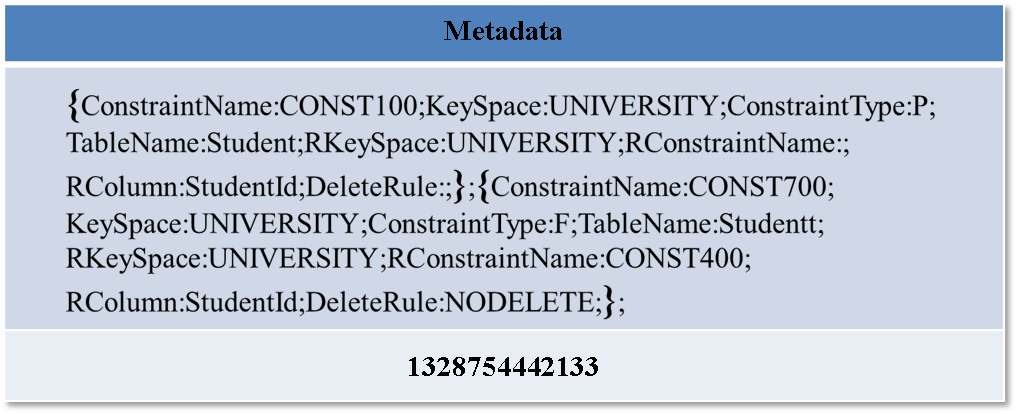
\includegraphics[width=1\textwidth]{./figure/Solutions/Sol1-MD-Col.png}
				\caption{Metadata Column in Solution 1}
				\label{fd:Metadata-Column}
	\end{figure}
	    

% 	
% 		\begin{figure}[h] \label{fd:Metadata-Solution1}
% 			\centering
% 			\subfigure[Metadata Column] {
% 				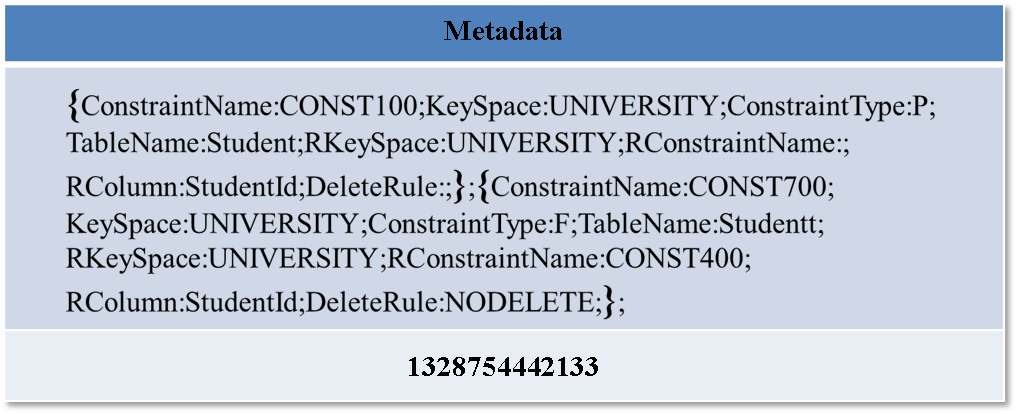
\includegraphics[width=.6\textwidth]{./figure/Solutions/Sol1-MD-Col.png}
% 				\label{fd:Metadata-Solution1-A}
% 	% 			\caption{Response Time for \texttt{insert}}\label{fr:response-insert}
% 			}
% 			\subfigure[Metadata in Super columns]{
% 				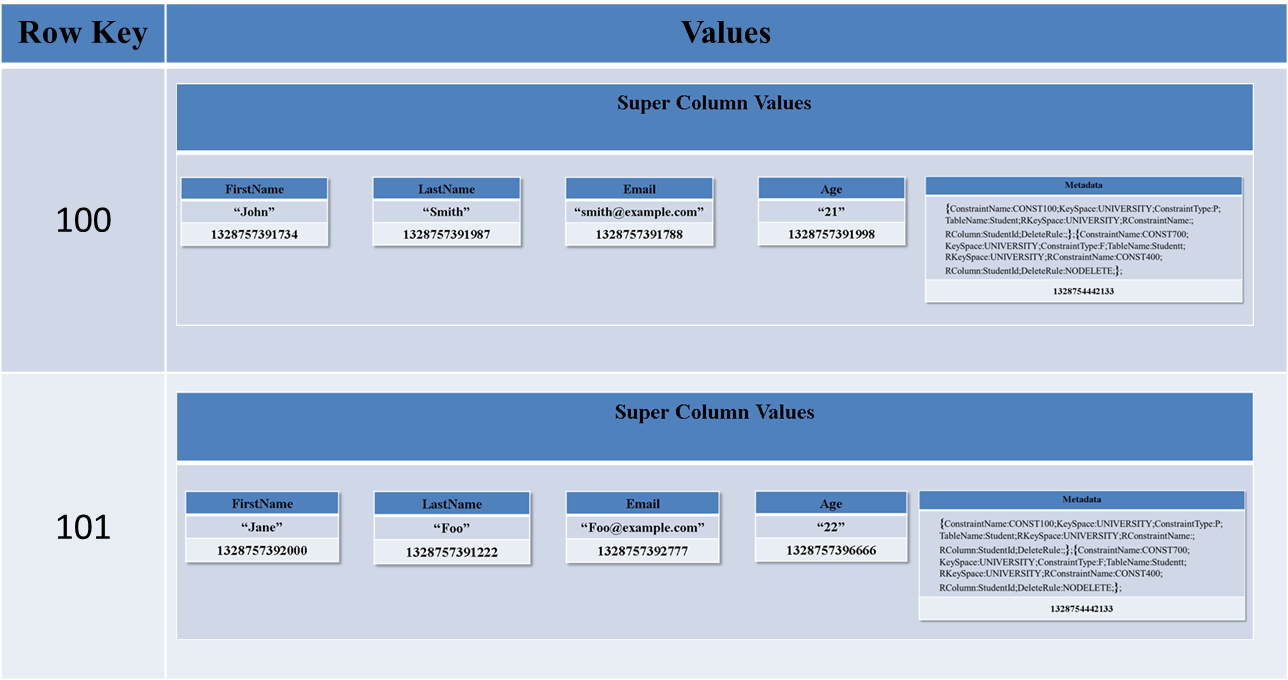
\includegraphics[width=.8\textwidth]{./figure/Solutions/Sol1-MD-ColumnFamily.png}
% 				\label{fd:Metadata-Solution1-B}
% 	% 			\caption{Throughput}\label{fr:through-insert}
% 			} 
% 			\caption{Metadata storage in Solution 1}
% 		\end{figure}
		
Since all the  constraints of a column family are saved together in the
\texttt{Metadata} column,  it is essential for each constraint to be easily
identifiable and accessible.  Thus, special characters are used within the
metadata to separate the constraints and to identify its different parts, as
shown in Figure~\ref{fd:Metadata-Column}. These characters are curly brackets
('\texttt{\{}', '\texttt{\}}') and semi-colon and colon ('\texttt{;}',
'\texttt{:}'). These special characters are used as follows.



% {\setlength{\fboxsep}{6pt}%
% \setlength{\fboxrule}{1pt}%
% 
% \fbox{\parbox{.9\linewidth}{\tt\centering
% % \{ConstraintName:CONST100;KeySpace:UNIVERSITY;ConstraintType:P;\\
% % TableName:Student;RKeySpace:UNIVERSITY;RConstraintName:;\\
% % RColumn:StudentId;DeleteRule:;\};\\
% \{ConstraintName:CONST700;KeySpace:UNIVERSITY;ConstraintType:F;\\
%  TableName:Studentt;RKeySpace:UNIVERSITY;RConstraintName:CONST400;\\
%  RColumn:StudentId;DeleteRule:NODELETE;\};\\
% }}
% }

% \vspace{12pt}

% The special characters :
	
		\begin{itemize}
			\item Each constraint is enclosed within curly brackets and the
			constraints are separated from each other with a
			'\texttt{;}'.  For example,  \texttt{CONST100} and \texttt{CONST200} are
			enclosed in curly braces and separated by '\texttt{;}'. 
			Thus,  '\texttt{\};}' marks the end of every constraint in the metadata. 
		
		
			\item The different parts in a constraint are separated by the special character
			'\texttt{;}'.  For example,  the \texttt{ConstraintName} and \texttt{Keyspace}
			and other parts in the constraints \texttt{CONST100} and \texttt{CONST200} are
			separated with a '\texttt{;}'.
			 
			 
			\item Each part and its respective value are separated by the special
			character '\texttt{:}'.  For example,  \texttt{ConstraintName} is separated from
			its value \texttt{CONST100} with a '\texttt{:}'.  
			
		\end{itemize}


% 

The special characters help in identifying the values of every constraint in the
metadata information for this solution. Thus, the metadata is extracted from
each super column and processed by specific methods within the solution so that
relevant constraints are used for validating referential integrity.  
% Different
% methods are built in the experimental \ac{API} to support these functionalities
% and these are described in Chapter~\ref{c:Implementation}. 

% In this solution,  the metadata is  repeated several times within the
% same column family and due to the replicated nature of the \ac{NoSQL} \acp{DBMS}
% the metadata is  stored several times across the nodes in the cluster.  This
% increases the redundancy of the metadata and much space would be consumed
% unnecessarily if the metadata is large.  

This design was inspired by the experiments done by~\citet{Hackl} on a popular
\ac{NoSQL} \ac{DBMS} named Tokyo Cabinet.  Tokyo Cabinet is similar to Cassandra
as data is stored in key-value pairs but it does not involve data types or
columns and column families as in Cassandra~\citep{Hackl,tokyo}.
% They proposed to store the metadata  information   stored in Tokyo Cabinet.
% In Hackl et al.   (2010),   metadata management is addressed in the context of
% huge file systems,  where metadata is stored separately in a suitable
% \ac{DBMS} so that such file systems can be managed and administered
% efficiently without slowing them down.   To analyse which type of \ac{DBMS}
% was more suitable for such a metadata storage,   they conducted various
% experiments and concluded that key-value \acp{DBMS} were more efficient in
% terms of speed,   memory and resource consumption when compared to popular
% \acp{RDBMS}.
As a part of their experiments to manage metadata for huge file systems,  they
adopted an approach to store metadata  as a part of the value in a key-value
pair.  In their approach, this value  is associated with a
unique key and the different parts of the metadata are separated by semicolons.
% where records are stored as simple key-value pairs in data files.
% In their approach,   metadata about the file system used in their experiment
% is inserted.
Their results showed that such a metadata storage provided high speed metadata
access where valuable information was integrated with the actual data.

Solution~1 derives this method of saving
metadata using special characters and integrating it with the actual data as
value in a key-value pair in Cassandra.  The metadata in this solution 
contains all the constraints pertinent to a keyspace and uses
the special characters to distinguish the relevant constraints and its various
parts.




\begin{landscape}
		\begin{figure}
			\centering
			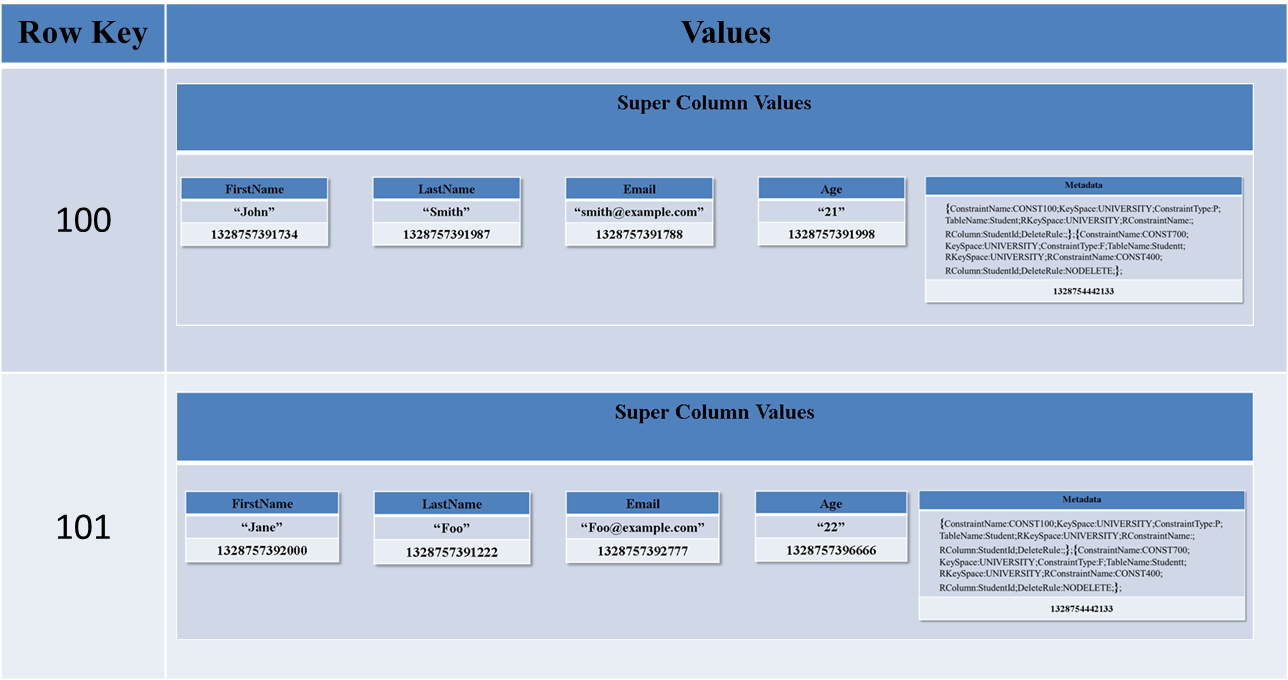
\includegraphics[width=1.4\textwidth]{./figure/Solutions/Sol1-MD-ColumnFamily.png}	
			\caption{Metadata in Solution 1}\label{fd:Metadata-Solution1}
			\end{figure}
		\end{landscape}










%ब

\section{Solution 2:  Metadata as a Top Row} \label{s:design-sol2}


In Solution~2,   metadata is embedded with the actual data and exists within the
same column family as the actual data, which is similar to Solution~1.
% where metadata is stored within the same column family.
However,  in this solution,   metadata is saved only once in the column family
as a top row. Specifically, it is stored in the first super column in a column
family) with the unique \texttt{RowId} '\texttt{-1}'.  This top row has only the
\texttt{Metadata} column which contains the metadata information as its value
while the rest of the super columns in the same column family have different
columns containing the actual data.  This design is possible since Cassandra
allows rows to have different number of columns within a column family.  The
\texttt{Metadata} column is similar to the Solution~1 as shown in
Figure~\ref{fd:Metadata-Column}.  Thus,  for each column family,  the metadata
exists only once as a single row and is common for all its super columns.  In
the University example, the  \texttt{Student} column family has the metadata 
stored as a top row as  shown in Figure~\ref{fd:Metadata-Solution2}.
% This approach helps preserve the dependency information while also making it
% easily accessible for the referential integrity validations.
		 
	\begin{figure}[h]  
		\centering 
		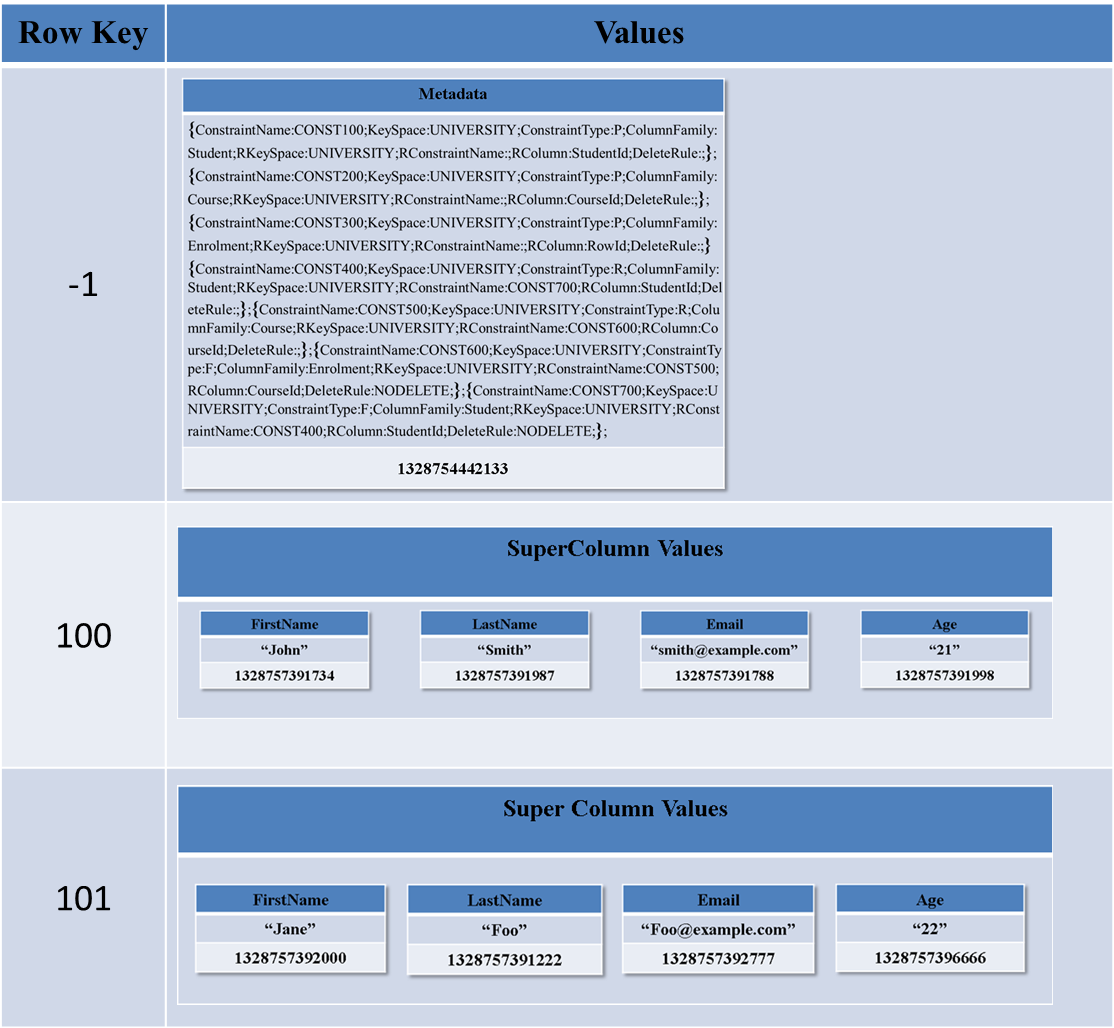
\includegraphics[width=.8\textwidth]{./figure/Solutions/Sol2-MD-ColumnFamily.png}
		\caption{Metadata storage in Solution 2}\label{fd:Metadata-Solution2}
	\end{figure}
		

In this solution, metadata  for each column family contains all the constraints
belonging to the keyspace. The metadata contains the same special characters
'\texttt{\{}',  '\texttt{\}}', '\texttt{;}' and '\texttt{:}' to distinguish all
the constraints and its different parts and values, as seen in
Solution~1. For example, the metadata for \texttt{Student}  contains
all the constraints as listed in Figure~\ref{fd:Metadata-Constraints} as its
metadata in the top row as shown in Figure~\ref{fd:Metadata-Solution2}.


% Consider \texttt{Enrolment}  which is a child entity with parent entities
% \texttt{Student} and \texttt{Course} (Figure~\ref{}).  Its metadata thus contains
% its \ac{PK} constraint \texttt{CONST300} and the \ac{FK} constraints
% \texttt{CONST400} and \texttt{CONST500}.  Since \texttt{Student} is a child
% entity it  stores its \ac{PK} constraint \texttt{CONST100} and its \ac{FK}
% constraint \texttt{CONST700}.  Similarly,  \texttt{Course} stores its \ac{PK} and
% respective \ac{FK} constraints. 
% 
% 	\begin{figure}
% 	\todo{ Insert metadata top row figure for Enrolment}
% 	\end{figure}
% 	Thus,  the metadats describes which is the
% 	primary key for the entity and the \ac{FK} constraints show which child entities dependent on the
% 	entity.  The \ac{FK} constraints are particularly useful to . 
	
The motivation behind this solution is to overcome the redundancy of metadata
storage in Solution~1 where  metadata is stored in every super column
of a column family and replicated across the cluster along with the column
family.  Solution~2 reduces this redundancy and centralises the metadata as a top
row within the column family.  Thus,  when metadata is large, lesser space is
consumed since it is not replicated as widely as in Solution~1. 
% In other words, the aim of this design was to reduce the redundancy of metadata in the column
% family whilst having metadata accessible to all the nodes by having it embedded
% with the actual data. 
Furthermore,  this solution  ensures that, when changes are made to the
metadata, the actual data is not accessed and only the
column family  is accessed to fetch the top row containing the metadata. 












%ब
\section{Solution3:  Metadata Column Family} \label{s:design-sol3}

In this approach,     metadata for all the column families in a keyspace is
stored in a separate column family called \texttt{Metadata}.   In this approach the metadata is
decoupled from the actual data and stored in a decentralised way where all the
\ac{PK} and \ac{FK} constraints of all the column families within a keyspace are
saved in a single location.  The other column families contain only the actual
data and does not store any metadata.  Using this approach,  all the constraints
as seen in Figure~\ref{fd:Metadata-Constraints} are saved as super columns in
the \texttt{Metadata} column family (Figure~\ref{fd:Metadata-Solution3}). 
 
	\begin{figure}[h] 
		\centering
		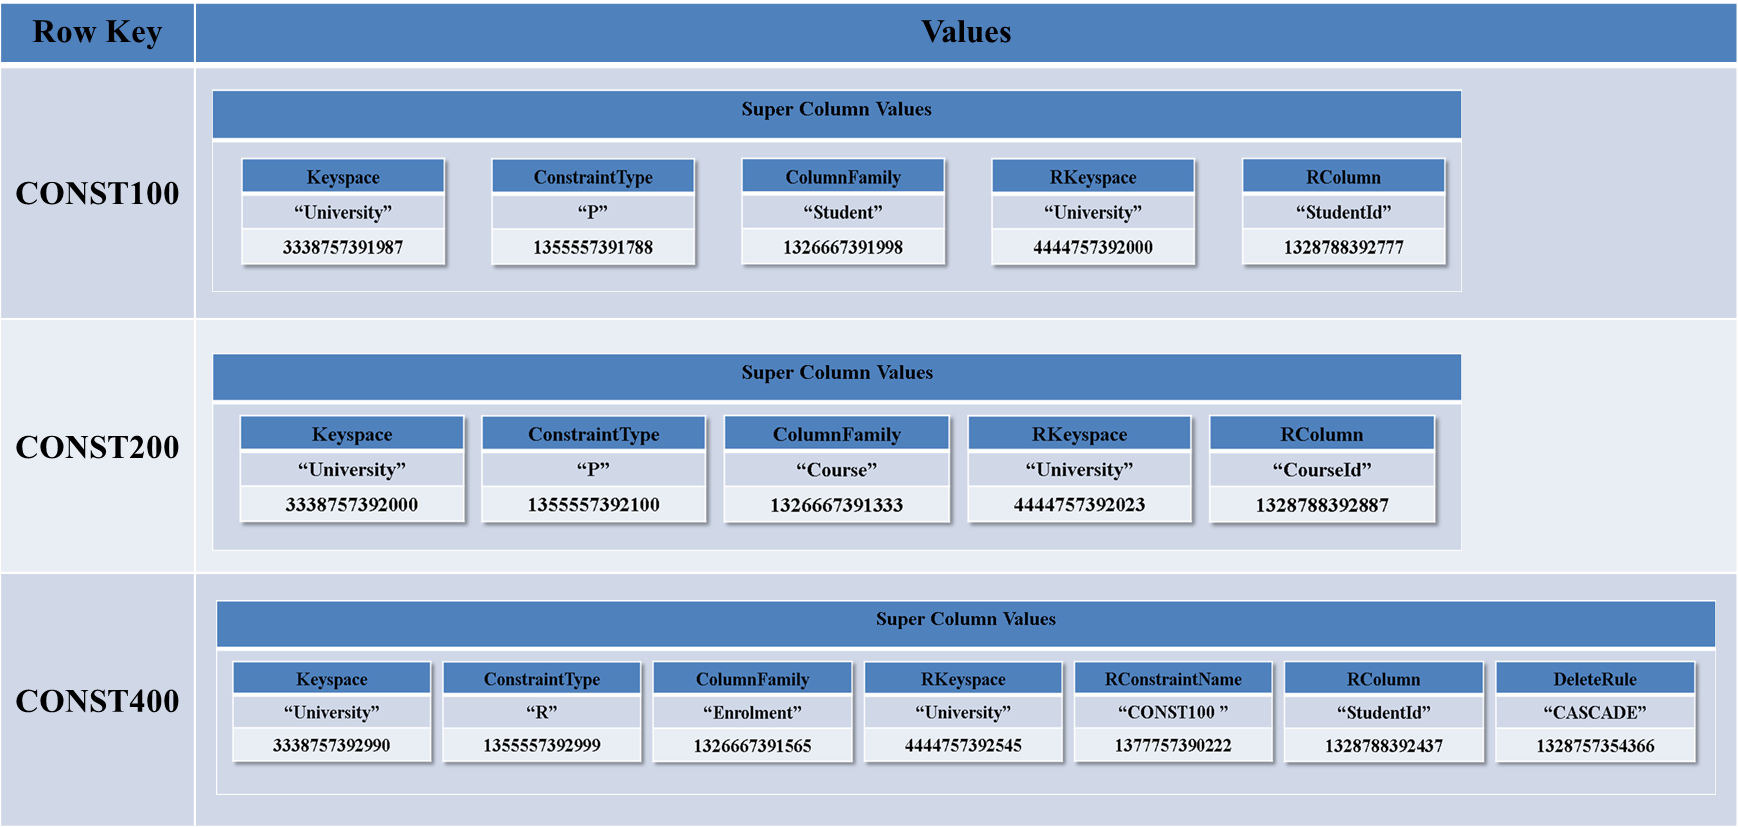
\includegraphics[width=.8\textwidth]{./figure/Solutions/Sol3-MD-ColumnFamily.png}
		\caption{Metadata Column Family in Solution 3}\label{fd:Metadata-Solution3}
	\end{figure}

The different parts of the constraints are saved as separate columns in the
\texttt{Metadata} column family. Thus,  no special characters are required to
identify the various parts as seen in Solutions~1 and 2.  When an operation is
invoked on a column family in the keyspace referential integrity validations
are triggered.  For these validations,  the experimental \ac{API} connects to
\texttt{Metadata} column family and retrieves the relevant constraints for the column family on
which the operation is invoked. 
The different parts of the constraints are accessed by identifying the
correct columns in the \texttt{Metadata} column family and necessary values are
retrieved to do the validation. 

This approach is similar to the way dependency information is
stored in traditional \acp{RDBMS},  where metadata holds information
about tables,  its dependencies and its many other properties.  Commonly,  such
metadata is maintained separately from the tables containing actual data and the
metadata is maintained in \texttt{System} tables.  
% Such tables  cannot be altered
% directly by the users and they can only query these tables for information. 
% Such an approach keeps metadata safe and away from users thus
% avoiding any mishandling of the metadata.  

The design to decouple metadata from the actual data is inspired from the
potential challenges in Solutions~1 and 2. 
% Such cases are when metadata undergoes frequent changes or a column family has
% many constraints. 
In Solutions~1 and 2,   a column family with several constraints will have a
large value in \texttt{Metadata} column and accessing as well as processing the
large metadata can consume more time.  Moreover,  in these solutions metadata has
to be changed at every place it is repeated in the event of any alterations to
the metadata. 
Consider Solution~1 where the \texttt{Metadata} column in every super column
of a column family has to be updated every time a constraint is added,  removed
or updated. 
In Solution~2,  the top row has to be changed for all the column families that have
any alterations  in their constraints.   

By decoupling metadata from the actual
data it is  easier to access and retrieve the various parts of the constraints
since these can be searched based on the column names once the constraint is
identified. 
More importantly,  it is now easier to add or remove constraints for a column
family since metadata  is centrally stored.  Any changes to metadata affects
only the \texttt{Metadata} column family and the experimental \ac{API} does not
have to access actual data to perform such changes. 


%ब
\section{Solution 4:  Metadata Cluster} \label{s:design-sol4}

In Solution~4,  metadata  is saved in a separate column family
similar to Solution~3. 
However,  in this solution,  the \texttt{Metadata} column family is saved in a
separate Cassandra cluster instead of saving it
within the same keyspace.  This means that the metadata storage
is decentralised and separated from the Cassandra cluster containing the
keyspace with actual data. 
Metadata  is not as widely replicated as in the previous solutions since the
replication of \texttt{Metadata} is only within the metadata cluster. 
Figure~\ref{fd:MetadataCluster-Solution4} shows an example of how the University
keyspace is saved in a separate cluster (nodes \texttt{A}, \texttt{B}, 
\texttt{C},  \texttt{D}) and the metadata is saved in the separate cluster called
Metadata cluster (nodes \texttt{L}, \texttt{M}, 
\texttt{N},  \texttt{O}).  
In this example,  the metadata column family \texttt{Metadata} is
inserted into \texttt{MetadataCluster},  while the column
families \texttt{Student},  \texttt{course} and \texttt{Enrolment} are entered
into another cluster,  namely \texttt{KeyspaceCluster}. 

% The Cassandra cluster is named ‘Test Cluster’ and consists
% of the nodes that have Cassandra with the entity column families (Student, 
% Course,  and Enrolment).  A separate cluster called “Metadata Cluster” consists of
% nodes that have only the metadata column families. 
\begin{figure}[h]
	\centering
	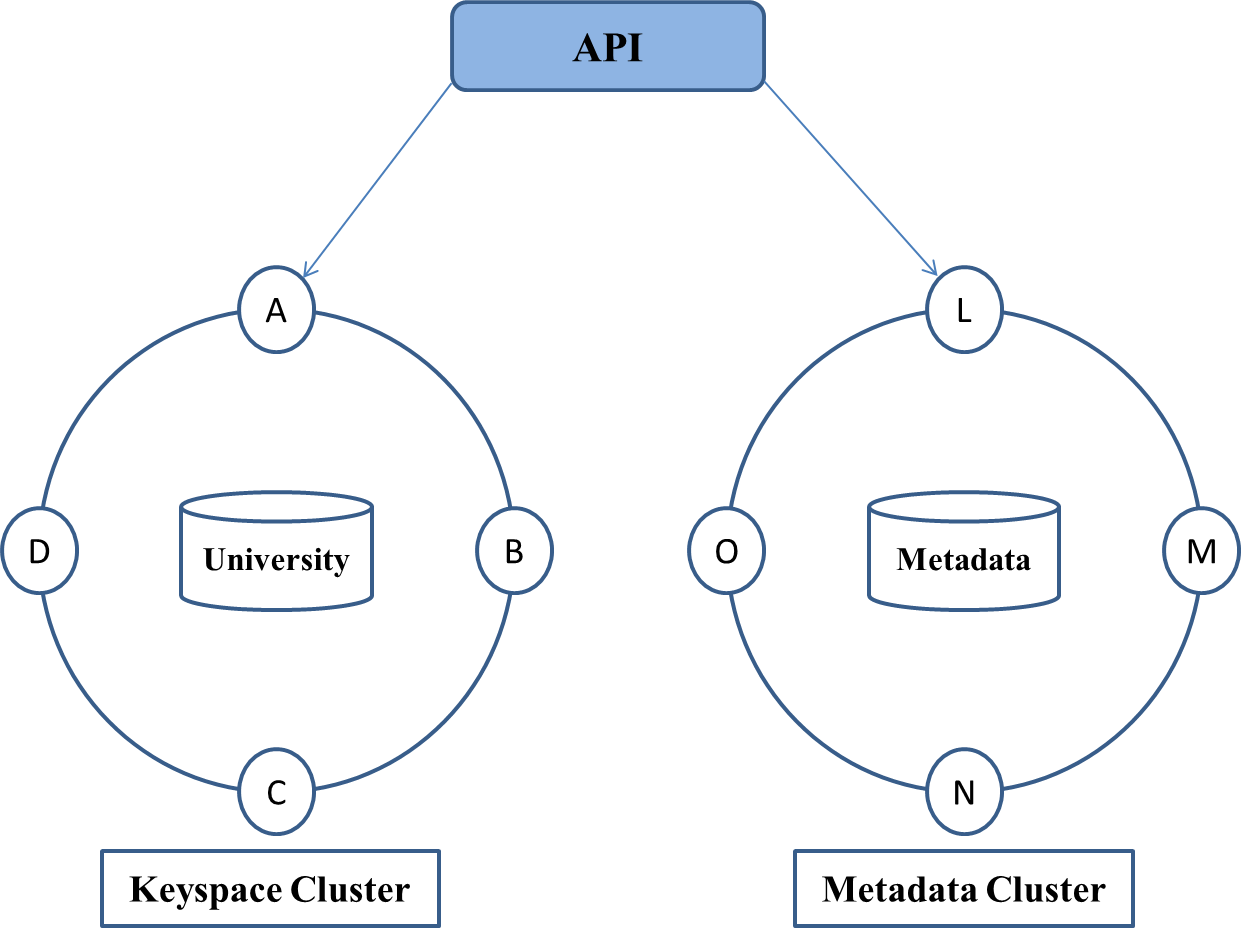
\includegraphics[width=.6\textwidth]{./figure/Solutions/Sol4-cluster-pic.png}
	\caption{Metadata Cluster in Solution
	4}\label{fd:MetadataCluster-Solution4}
	
\end{figure}
 The experimental \ac{API} connects to the Metadata cluster as well as
the cluster containing the keyspace to perform any operations on the actual
data.  Whenever a \ac{CRUD} operation is invoked on a column family,  the
experimental \ac{API} accesses its relevant metadata and caches it to re-use it
for future operations on this column family. 
Additionally, if the metadata cluster becomes unresponsive or not active,  the
experimental \ac{API} can continue performing validations despite such
disruptions using the cached metadata.
Having metadata cached is effective since metadata is not
expected to be as frequently changed as the actual data.  This also saves
operational time by not having to connect to the
\texttt{Metadata} column family each time  metadata is accessed. 


% As of now,  ‘Test Cluster’ is the name of the cluster for all the entity column
% families existing on Cassandra nodes.  Some of the Cassandra nodes are
% Saddleback,  meow,  Marrakech etc.  located in the ECS labs.  To have a separate
% cluster of nodes for Metadata,  it was required that the Cassandra configuration
% files were changed.  This involved changing the listening port,  RPC port,  and TCP
% port to different values from that of the ‘Test Cluster’.  It was also necessary
% to change the path configurations for the saved caches and log files so that it
% does not overwrite the files of the ‘Test Cluster’. 


% Just as in other solutions,  metadata information needs to be checked during
% any database operations.  Every time a referential integrity check is
% performed,  the API connects to the ‘Metadata Cluster’ and retrieves the
% metadata information. 
% Connection pools are maintained to reuse the connections whenever needed.  In
% order to perform the database operations,  the API then connects to the ‘Test
% Cluster’ on any of its nodes.  For example,  if an insert operation is invoked
% on Enrolment,  it is necessary to check if the foreign keys for Student and
% Course column families exist in their respective parent column families.  The
% details of the referenced column families are retrieved from the Metadata
% column family in the ‘Metadata Cluster’.  Once this information is processed, 
% the API connects to the referencing column families in the ‘Test Cluster’ and
% completes the insert operation. 
This  approach is useful when an application handles multiple keyspaces
and have to store and maintain large amounts of metadata  for  several
keyspaces. 
In such cases it is straightforward  to maintain all the metadata  in a
separate cluster  decoupled from the actual data and avoids having to handle
the actual data. 
% Even if the metadata
% cluster is unresponsive or not active the \ac{API} can perform operations with 
% the cached metadata. 
 
 This approach is inspired from the way most distributed systems save metadata
 in Metadata Server clusters~\citep{bin-et-al,Fu,lin}.
 For better scalability and efficient access of metadata,  these clusters are
 often separately maintained in large distributed environments where a master
 metadata server and subordinate metadata servers handle various
 responsibilities within the cluster.
 In Solution~4 such delegations of tasks are not required since all nodes in a
 Cassandra cluster  have the same responsibilities and do not have a
 master-slave configuration.  Thus, Solution~4  adopts the design of having
 a cluster of dedicated nodes to save metadata information and to have a central
 location to preserve and maintain metadata for many keyspaces.
 



\section{Summary}\label{s:Design-summary}
The main difference in the design of all the  solutions is the way each of the
solutions store metadata.    Solution~1 stores metadata with the data in every
super column providing fast access to the metadata but increasing its
redundancy. 
Solution~2 has a similar approach as Solution~1 but stores metadata in a single
super column in every column family.   This approach is useful when the metadata
is large since it consumes less space when compared to Solution~1. 
Both Solutions~1 and 2 use special characters in the metadata in order to
distinguish the  constraints relevant to an entity. 
Solution~3 separates the metadata from the actual data and stores all the
constraints together for all column families of a keyspace  in a centralised
way.    This is useful when metadata has to be  altered because it simplifies the
management of metadata.  
Solution~4 has a similar approach as Solution~3,  but saves the \texttt{Metadata}
column family in a separate cluster on different nodes.    It also caches the
metadata  to save operational time and reduce database connections to a
different cluster. 

The next chapter presents the  experimental \ac{API} which provides methods for
 retrieving and processing the metadata as well as handling all the \ac{CRUD}
 operations and referential integrity validations.  

% Since metadata storage is unique in each  solution,  The way metadata is accessed
% and processed are different in each of the solutions.   
%  As mentioned previously,  the experimental \ac{API} provides methods for
%  retrieving and processing the metadata and  handles all the \ac{CRUD}
%  operations as well as the referential integrity validations.  This is 
%  discussed in the next chapter.  

% Thus,   this
% solution differs from Solution~1 only in the way the metadata is stored to improve resource
% utilisation and the way special characters are used and saving only the
% relevant constraints for a column family are  the same as in Solution~1.   
% It also explains how each of the solutions retrieves and processes the
% metadata.   

% The insert,   update and delete operations are performed similar to the other
% solutions.   


% These methods and all the
% solutions are incorporated  into an experimental \ac{API},   which is
% described in Chapter~\ref{c:Implementation}.   
